\begin{tcolorbox}
Die Produktfunktionen beschreiben jede einzelne Funktion des Produkts mittels Anwendungsfalldiagrammen und Anwendungsfalltabellen.
Diese sollen möglichst ausschlaggebend für das zu entwickelnde System sein und nicht simple Produktfunktionen wie z.B. Login, Account erstellen, Gruppe beitreten, Passwort ändern oder ähnliches zeigen.
\autoref{fig:anwendungsfall-app-tabelle-xx-1} stellt eine exemplarische Tabelle für die Beschreibung eines Anwendungsfalls dar. Stil und Formatierung sind variabel. Nicht jede Zelle muss immer gefüllt sein.
\\\\
In  Tabelle~\autoref{fig:akteur-tabelle} werden alle auftretenden Akteure beschrieben.


\end{tcolorbox}

\begin{figure}[h]
	\centering
	
	\begin{tabularx}{\textwidth}{ p{.2\textwidth} | p{.2\textwidth} | X }
		\textbf{Akteur} & \textbf{Beschreibung} & \textbf{Verwendet in Anwendungsfall} \\ \hline
		Informatiker & Programmiert tolle Sachen & Programmieren, Kaffee trinken, Schlafen
	\end{tabularx}
	
	\caption{Beschreibung der Akteure}
	\label{fig:akteur-tabelle}
\end{figure}

\newpage

\section{Anwendungsfalldiagramm - App}

\begin{figure}[h]
	\centering
    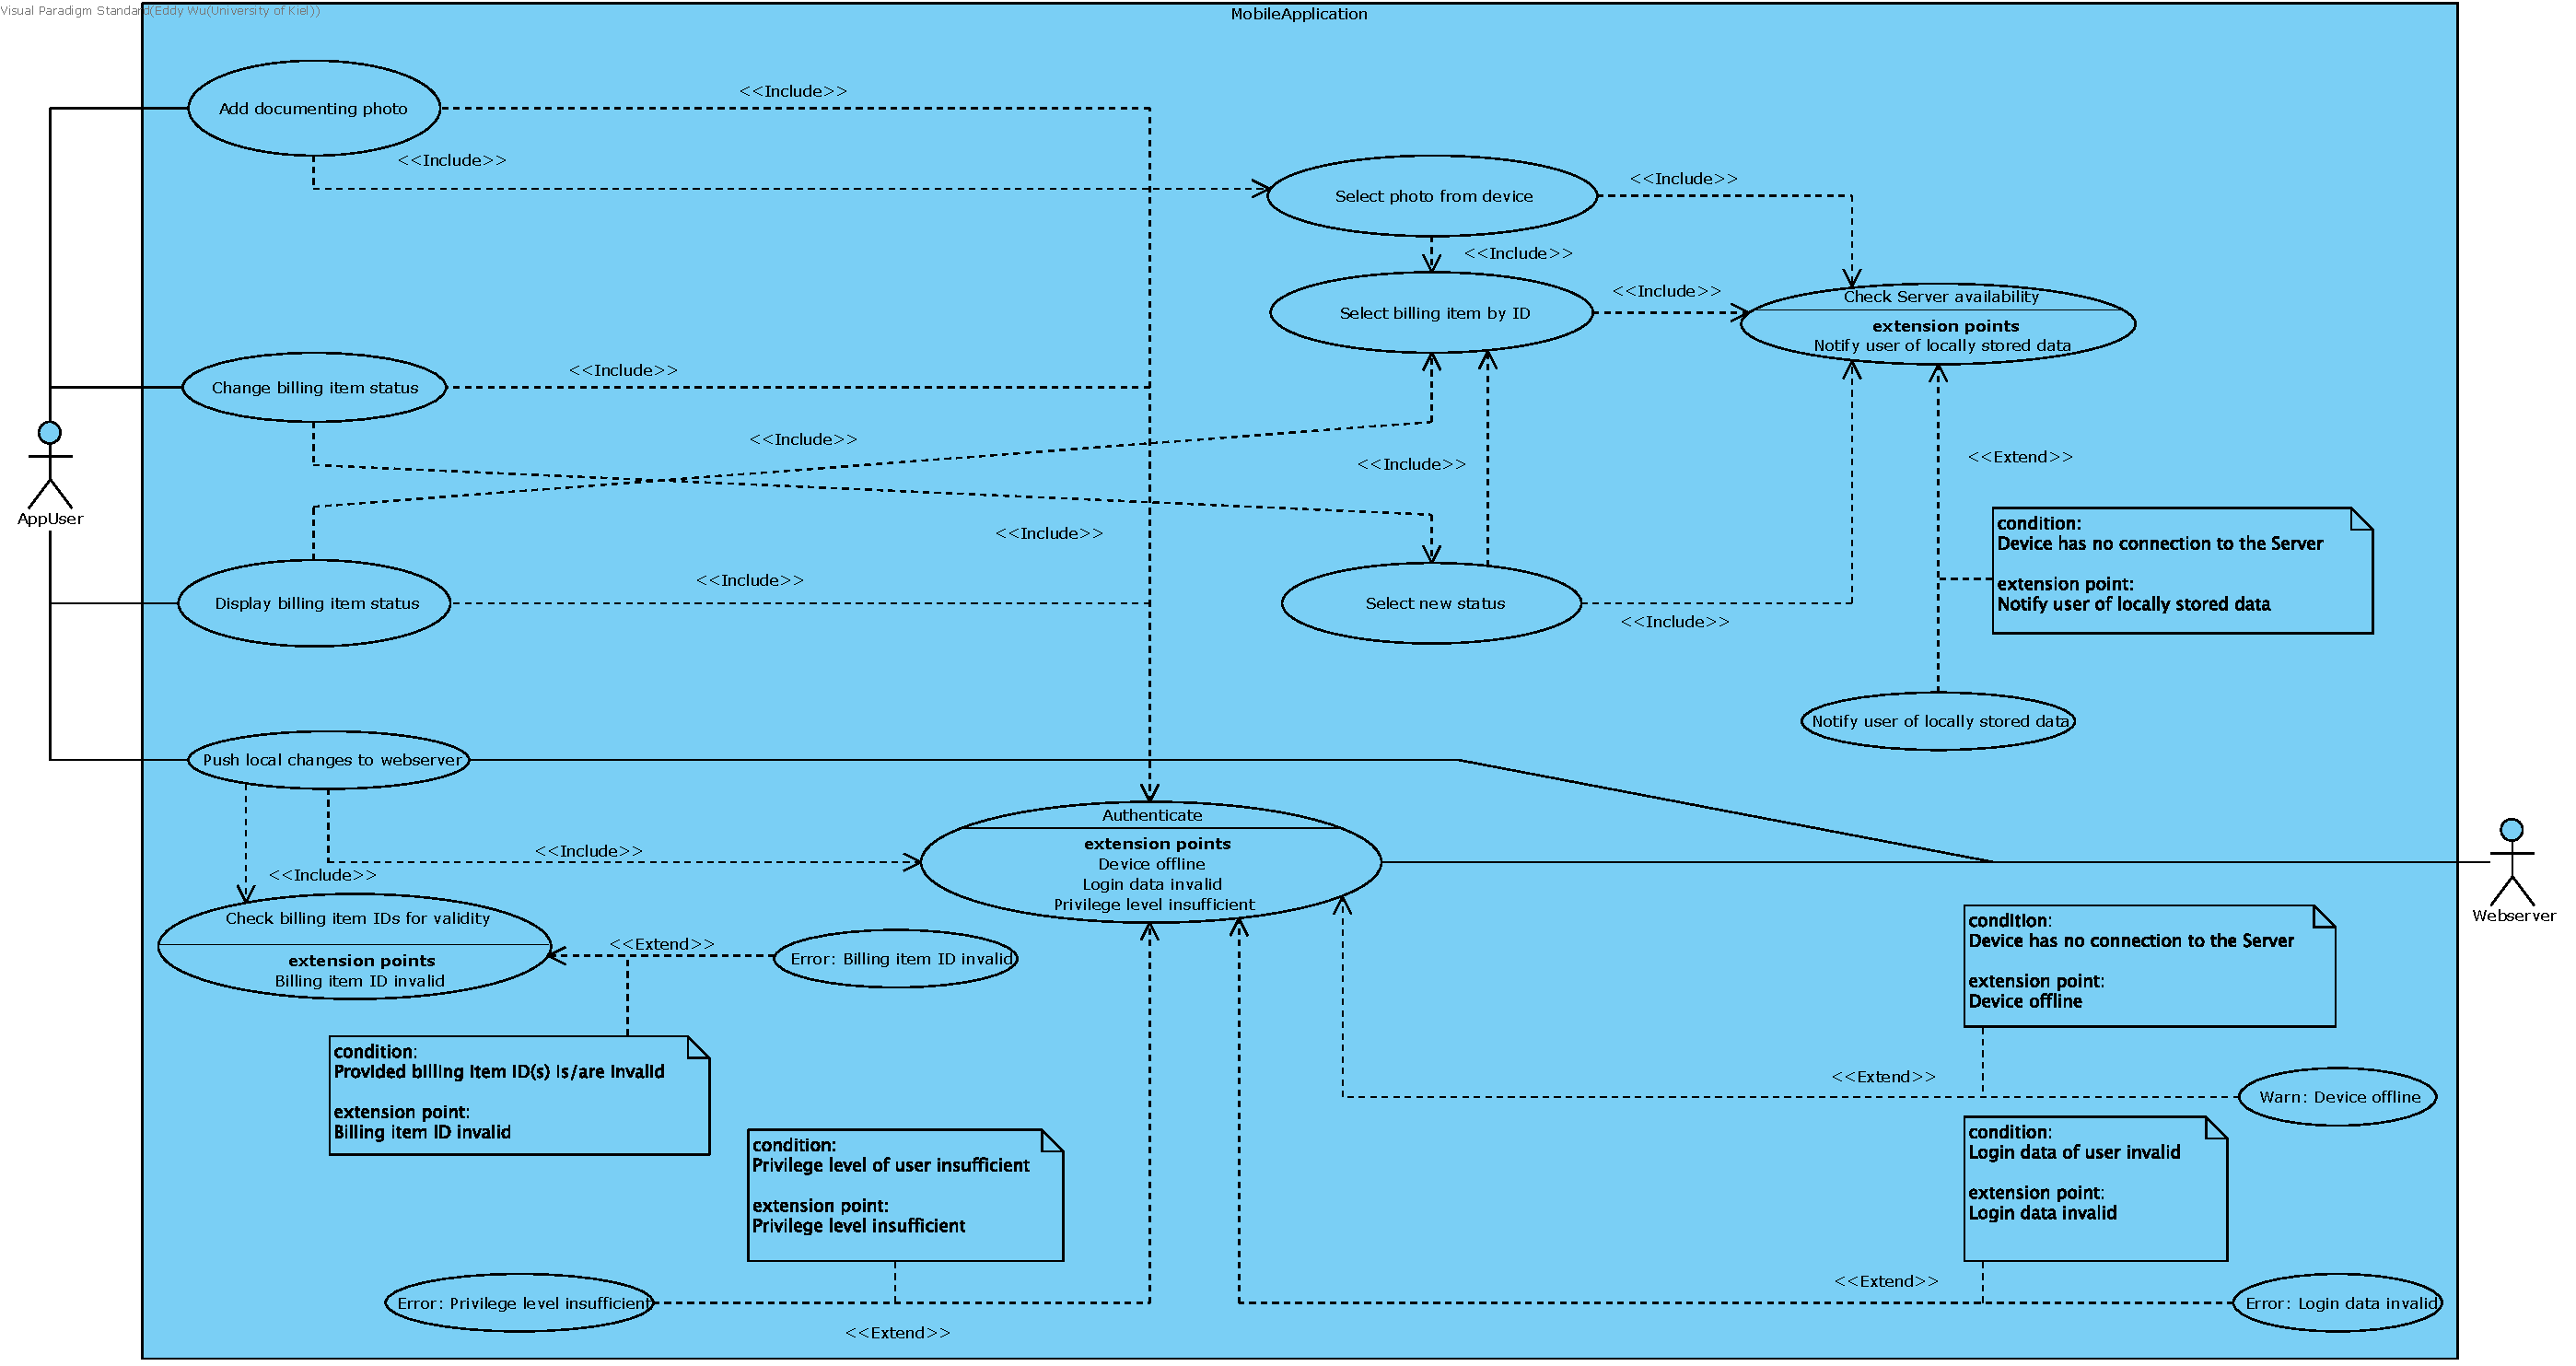
\includegraphics[width=\linewidth]{img/diagrams/Mobile_Application.pdf}
	\caption{Anwendungsfalldiagramm - App}
	\label{fig:anwendungsfalldiagramm-app}
\end{figure}

\newpage

\begin{figure}[h]
	\centering
	\begin{tabularx}{\textwidth}{ X | X }
		\textbf{Anwendungsfall ID} & APP-1 \\ \hline
		\textbf{Anwendungsfallname} & Push local changes to webserver\\ \hline
		\textbf{Initiierender Akteur} & AppUser \\ \hline
		\textbf{Weitere Akteure} & Webserver  \\ \hline
		\textbf{Kurzbeschreibung} & Der Benutzer der Applikation kann lokale \"Anderungen,  bspw. \"Anderungen zum Baustatus einzelner Leistungspositionen oder Fotos mit Kommentar von der Baustelle,  an den Webserver schicken.  Diese \"Anderungen und Fotos mit Kommentar k\"onnen dann enstprechend  \"uber die Webanwendung eingesehen werden.  \\ \hline
		\textbf{Vorbedingungen} & Der AppUser ist registriert und entsprechend eingeloggt \\ \hline
		\textbf{Nachbedingungen} & Die lokalen Daten wurden an den Webserver geschickt\\ \hline
		\textbf{Ablauf} &
			\begin{enumerate}
				\item Der AppUser hat den Status einer Leistungspositionen  lokal ge\"andert.
				\item Der Benutzer verwendet die Funktion der App,  um seine lokale \"Anderung an den Webserver zu \"ubertragen.
				\item Es besteht eine Internetverbindung und der AppUser erh\"alt die R\"uckmeldung,  dass das Vorhaben erfolgreich ausgef\"uhrt wurde.  
				\item Die \"Anderung befindet sich nun auf dem Webserver.
			\end{enumerate}
			\end{tabularx}
	\caption{Anwendungsfall APP-1}
	\label{fig:anwendungsfall-app-tabelle-APP-1-1}
\end{figure}
			\begin{figure}[h]
	\centering
	\begin{tabularx}{\textwidth}{ X | X }
		\textbf{Alternative} & 
				\begin{enumerate}
					 \item Der AppUser hat seinen Benutzerrechten entsprechend ein Foto zur Dokumentation einer Leistungsposition angefertigt.
					 \item Das Foto soll nun durch Bet\"atigen der entsprechenden Funktion der mobilen Applikation auf den Webserver hochgeladen werden.
					 \item Es besteht eine Internetverbindung und der AppUser erh\"alt eine entsprechende Meldung,  dass der Upload erfolgt.
					 \item Das Foto wird an den Webserver \"ubertragen.
				\end{enumerate}  \\ \hline
						\textbf{Ausnahme} &
				\begin{enumerate}
					 \item Der AppUser m\"ochte eine \"Anderung an dem Status einer Leistungsposition oder ein Foto zur Dokumentation mit Kommentar an den Webserver \"ubertragen und verwendet die enstprechende Funktionalit\"at der Applikation.
					 \item Der User erh\"alt eine Fehlermeldung, da seine Rechte nicht ausreichen um diese Aktion durchzuf\"uhren.
					 \item Die \"Anderungen am Status der Leistungsposition und/oder das Foto mit Kommentar werden nicht an den Webserver \"ubertragen.
					 \end{enumerate} \\ \hline
	\end{tabularx}
	\caption{Anwendungsfall APP-1}
	\label{fig:anwendungsfall-app-tabelle-APP-1-2}
\end{figure}
			\begin{figure}[h]
	\centering
	\begin{tabularx}{\textwidth}{ X | X }
					 	\textbf{Ausnahme} &
				\begin{enumerate}
					\item Die lokalen \"Anderungen durch den Benutzer sollen durch Bet\"atigung der entsprechenden Funktion in der App an den Webserver \"ubertragen werden.
					\item Der AppUser erh\"alt eine Fehlermeldung,  da zur Zeit f\"ur das verwendetete Ger\"at keine (ausreichende) Internetverbindung besteht. 
					\item Der Benutzer erh\"alt eine R\"uckmeldung,  dass zur Zeit keine Internetverbindung besteht und lokale \"Anderungen zwischengespeichert werden.
					\item Sobald eine ausreichende Internetverbindung besteht,  werden die entsprechenden Daten an den Webserver \"ubertragen.
				\end{enumerate} 
				 	\end{tabularx}
	\caption{Anwendungsfall APP-1}
	\label{fig:anwendungsfall-app-tabelle-APP-1-3}
\end{figure}
			\begin{figure}[h]
	\centering
	\begin{tabularx}{\textwidth}{ X | X }
		\textbf{Ausnahme} &
				\begin{enumerate}
				\item Der Benutzer loggt sich innerhalb der App mit seinen registrierten Benutzerdaten, bestehend aus Benutzername und Passwort,  ein.  
					 \item Der AppUser m\"ochte eine \"Anderung an dem Status einer Leistungsposition an den Webserver \"ubertragen und verwendet die entsprechende Funktion in der Applikation. 
					 \item Die Identifikationsnummer der betroffenen Leistungsposition ist nicht g\"ultig.
					 \item Der User erh\"alt eine Fehlermeldung.
					 \item Die \"Anderungen am Status der Leistungsposition werden nicht an den Webserver \"ubertragen.
				\end{enumerate} \\ \hline
						\textbf{Ausnahme} &
				\begin{enumerate}
					 \item Der AppUser m\"ochte eine lokale \"Anderung an dem Status einer Leistungsposition oder ein Foto mit Kommentar an den Webserver \"ubertragen und verwendet die entsprechende Funktion in der Applikation. 
					 \item Die Identifikationsnummer der betroffenen Leistungsposition ist nicht g\"ultig.
					 \item Der User erh\"alt eine Fehlermeldung.
					 \item Die \"Anderungen am Status der Leistungsposition oder das Foto mit Kommentar werden nicht an den Webserver \"ubertragen.
				\end{enumerate} \\ \hline
		\textbf{Benutzte Anwendungsfälle} & Authenticate,  Check BillingItemIDs for validity\\ \hline
		\textbf{Spezielle Anforderungen} & - \\ \hline
		\textbf{Annahmen} & -
	\end{tabularx}
	\caption{Anwendungsfall APP-1}
	\label{fig:anwendungsfall-app-tabelle-APP-1-4}
\end{figure}

\clearpage

\section{Anwendungsfalldiagramme - Webserver}

\subsection{Account-Management}

\begin{figure}[h]
	\centering
	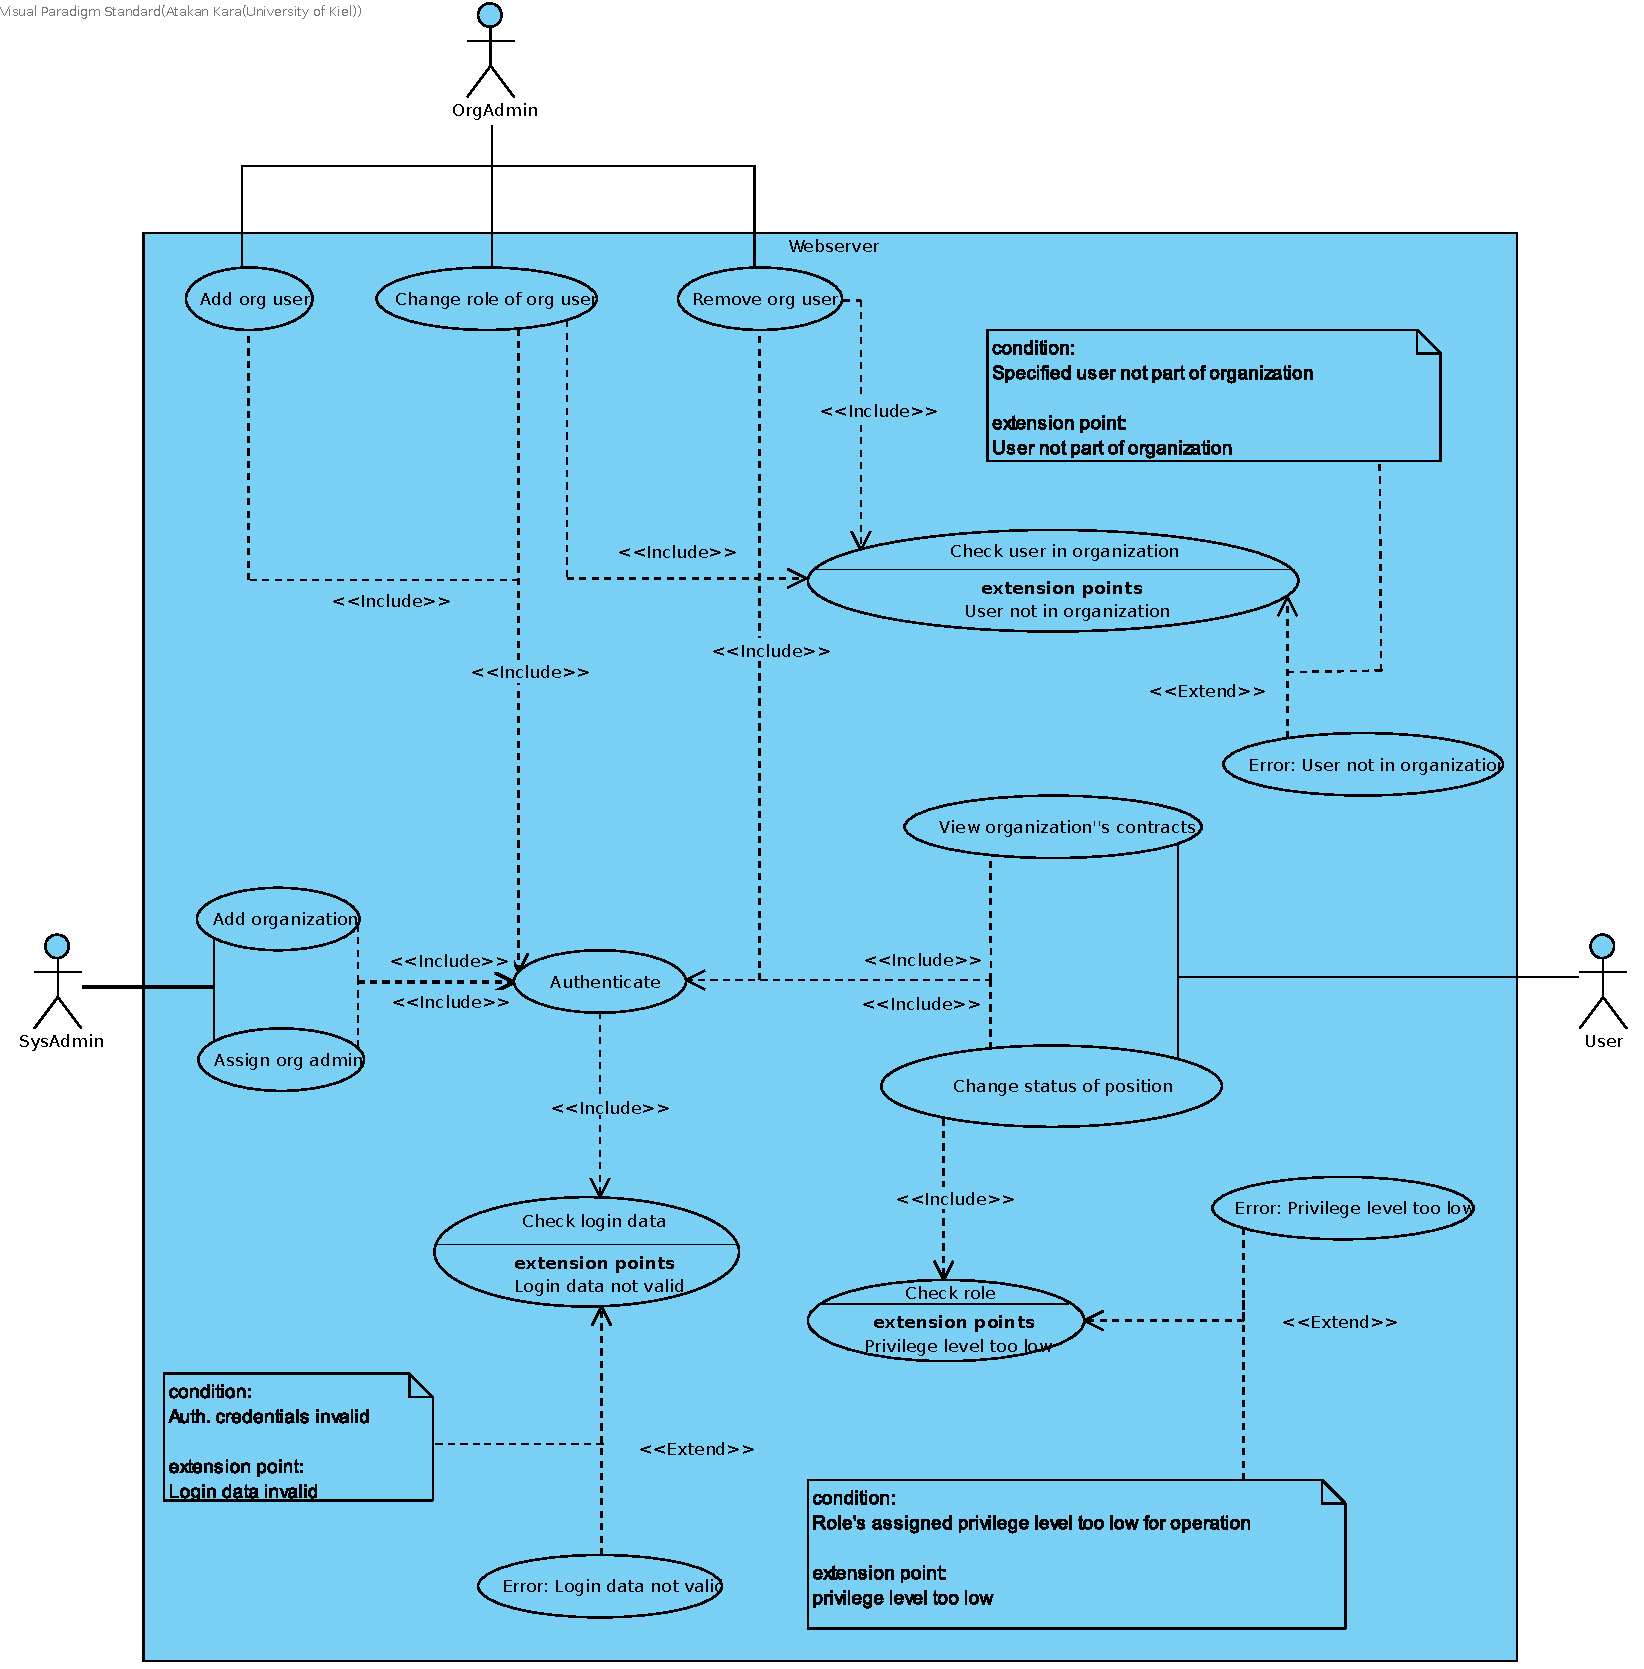
\includegraphics[width=\linewidth]{img/diagrams/Acc_Management_Web.pdf}
	\caption{Anwendungsfalldiagramm - Account-Management Webserver}
	\label{fig:anwendungsfalldiagramm-acc}
\end{figure}

\newpage

\begin{figure}[h]
	\centering
	\begin{tabularx}{\textwidth}{ X | X }
		\textbf{Anwendungsfall ID} & ACC-1 \\ \hline
		\textbf{Anwendungsfallname} & Change status of position\\ \hline
		\textbf{Initiierender Akteur} & User \\ \hline
		\textbf{Weitere Akteure} & -  \\ \hline
		\textbf{Kurzbeschreibung} & Der User kann den Satus von Leistungspositionen ver\"andern \\ \hline
		\textbf{Vorbedingungen} & User ist entsprechend eingeloggt, Rechte des Users sind ausreichend f\"ur diese Operation \\ \hline
		\textbf{Nachbedingungen} & Status wurde ver\"andert \\ \hline
		\textbf{Ablauf} &
		\begin{enumerate}
			\item Der User \"andert den Status einer Leistungsposition und w\"ahlt die entsprechende Funktion der Weboberfl\"ache, dass diese \"Anderung \"ubernommen werden sollen.
			\item Die Aktion war erfolgreich und die \"Anderung wurde \"ubernommen.  Der User erh\"alt eine R\"uckmeldung \"uber den Erfolg der Aktion.
		\end{enumerate} \\ \hline
		\textbf{Alternative} & -
		\\ \hline
		\textbf{Ausnahme} &
		\begin{enumerate}
			\item Der User \"andert den Status einer Leistungsposition und w\"ahlt die entsprechende Funktion der Weboberfl\"ache,  dass diese \"Anderung \"ubernommen werden sollen.
			\item Der User verf\"ugt nicht \"uber die entsprechenden Rechte die Aktion durchzuf\"uhren und erh\"alt eine Fehlermeldung. Der bisherige Status der Leistungsposition bleibt bestehen.
		\end{enumerate}  \\ \hline
		\textbf{Benutzte Anwendungsfälle} & Authenticate \\ \hline
		\textbf{Spezielle Anforderungen} & - \\ \hline
		\textbf{Annahmen} & -
	\end{tabularx}
	\caption{Anwendungsfall ACC-1}
	\label{fig:anwendungsfall-server-tabelle-ACC-1}
\end{figure}

\clearpage

\subsection{Diagrammdarstellung}

\begin{figure}[h]
	\centering
	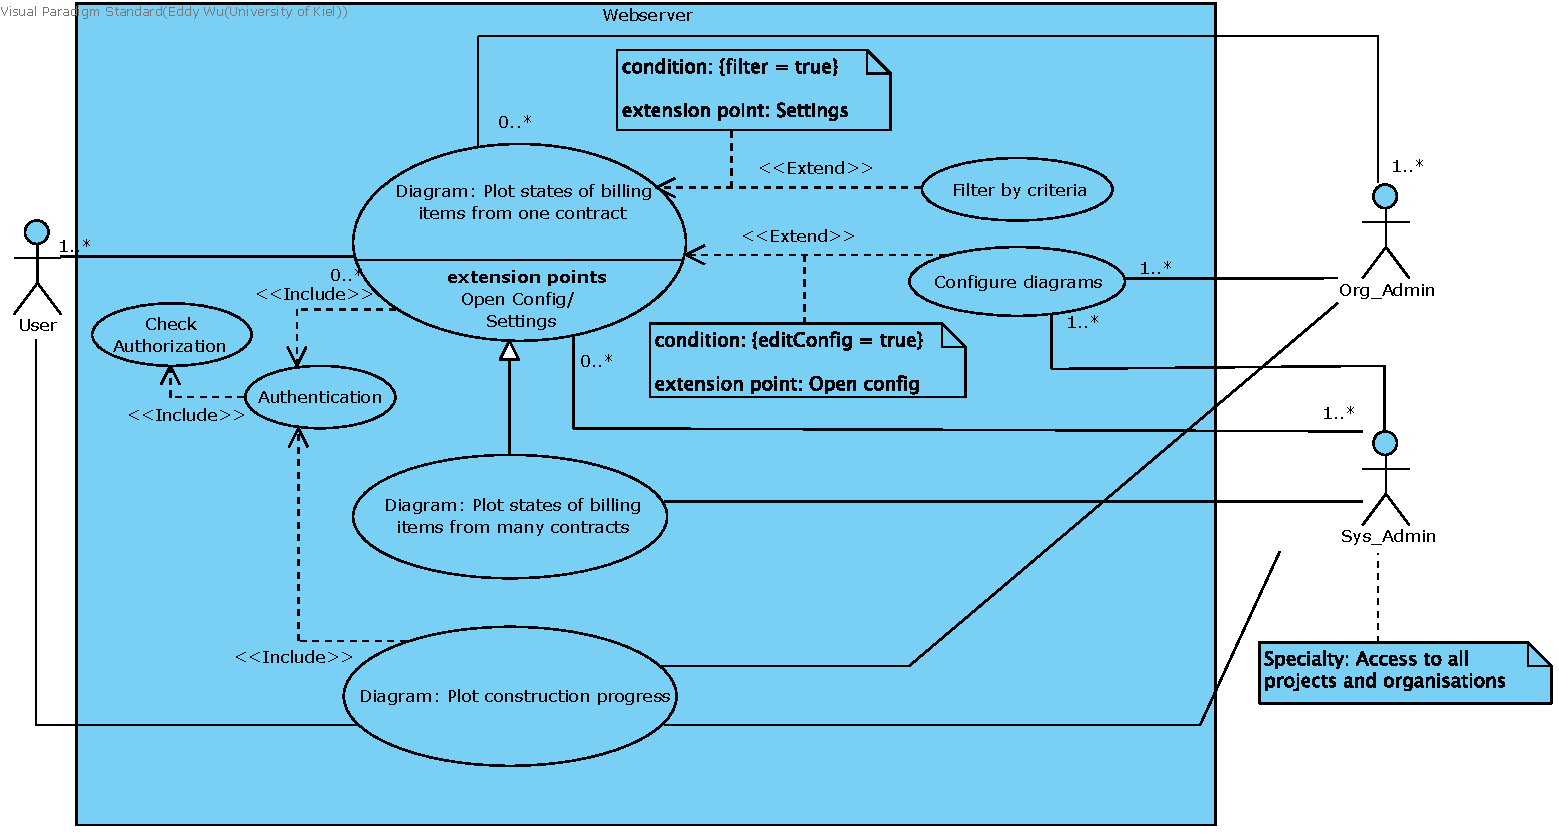
\includegraphics[width=\linewidth]{img/diagrams/Diagram_Display_Management_Web.pdf}
	\caption{Anwendungsfalldiagramm - Diagrammdarstellung}
	\label{fig:anwendungsfalldiagramm-dia-management}
\end{figure}

\newpage

\begin{figure}[h]
	\centering
	\begin{tabularx}{\textwidth}{ X | X }
		\textbf{Anwendungsfall ID} & DIA-1 \\ \hline
		\textbf{Anwendungsfallname} & Diagrammverwaltung \\ \hline
		\textbf{Initiierender Akteur} & Systemadministrator \\ \hline
		\textbf{Weitere Akteure} & Organisationsadministrator, Mitarbeiter \\ \hline
		\textbf{Kurzbeschreibung} & Darstellung und mögliche Filterung der vom Server automatisch erzeugten Diagramme innerhalb der Webapplikation.  \\ \hline
		\textbf{Vorbedingungen} & Funktionierende Internetverbindung, bestätigte Berechtigungen (Authentifiziert)  \\ \hline
		\textbf{Nachbedingungen} &  -  \\ \hline
		\textbf{Ablauf} &
		\begin{enumerate}
			\item Authentifizieren.
			\item Darstellen eines allgemeinen (alle Leistungspunkte umfassend) Diagramms zu einem oder mehreren Verträgen.
		\end{enumerate} \\ \hline
		\multirow{2}{*}{\textbf{Alternativen}} &
		%%\textbf{Alternative} &
		\begin{enumerate}
			\item Authentifizieren.
			\item Filtern nach bestimmten Kriterien.
			\item Darstellen eines Diagramms zu einem oder mehreren Verträgen.
		\end{enumerate} \\\cline{2-2} &
		\begin{enumerate}
			\item Authentifizieren.
			\item Diagramm zum Baufortschritt eines Projektes anzeigen.
		\end{enumerate}  \\ \hline
		%%\textbf{Ausnahme} &
		\multirow{2}{*}{\textbf{Ausnahme}} &
		\begin{enumerate} % Projekt/Vertrag nicht vorhanden.
			\item Authentifizieren.
			\item Diagramm zum Baufortschritt eines nicht-existenten Projektes anzeigen.
			\item Fehlermeldung!
		\end{enumerate} \\\cline{2-2} &
		\begin{enumerate} % Fehlende Berechtigungen.
			\item Authentifizieren.
			\item Diagramm ohne passende Rolle anzeigen lassen.
			\item Fehlermeldung!
		\end{enumerate}  \\ \hline
		\textbf{Benutzte Anwendungsfälle} & Benutzerverwaltung (ACC-1) \\ \hline
		\textbf{Spezielle Anforderungen} & - \\ \hline
		\textbf{Annahmen} & -
	\end{tabularx}
	\caption{Anwendungsfall DIA-1}
	\label{fig:anwendungsfall-diagrammverwaltung-tabelle-DIA-1}
\end{figure}